% !TEX root = ../thesis.tex
% current project state
% @author Tobias Wulf
%

\section{Stand der Vorarbeiten}\label{sec:stand-der-vorarbeiten}

Zur Erörterung der Ziele und Inhalte dieser Arbeit, findet einleitend eine kurze Zusammenfassung der Vorarbeiten statt.
Für den Inhalt relevante Aspekte der Vorarbeiten werden im \autoref{ch:grundlagen} näher beleuchtet und erklärt.
\newline
Aktuell steht kein magnetisches TMR-Sensor-Array als integrierte Lösung zur Verfügung. Im Zuge des Forschungsprojekts Signalverarbeitung für \gls{ac:isar} sind in der \gls{gl:ags} Machbarkeitsstudien erbracht worden \cite{Mehm2019}\cite{Ernsting2020}. Zielstellung war dabei die Untersuchung der generellen Funktionalität und technischen Umsetzung eines magnetischen Sensor-Arrays im Maßstabsmodell.


\paragraph{Platinen-Sensor-Array}\label{par:platinen-sensor-array}$~$\\


Für den Aufbau des Platinen-Sensor-Arrays sind einzelne Winkelsensoren in Sensorbänken angeordnet, \autoref{fig:sensor-array-platine-8x8}. Die Messwerterfassung erfolgt über ein Multiplexing-Verfahren. Eine Steuerung des Multiplexings und die weitere Messwertverarbeitung erfolgt mit Hilfe eines Mikrocontrollers.

Diese Herangehensweise lässt eine Untersuchung der technischen Machbarkeit auf der Basis von aktuell verfügbaren Technologien und Winkelsensoren zu.
So ist das Platinen-Sensor-Array in verschieden Versionen, mit \gls{ac:amr}-Sensoren der Firma NXP Semiconductors 
(KMZ60) \cite{NXPSemiconductors2014} und TMR-Sensoren der Firma TDK (TAS2141-AAAB) \cite{TDK2016} verwirklicht worden. 
Das Maßstabsmodell des magnetischen Sensor-Arrays kann zu Vergleichs- und weiteren Erprobungsarbeiten genutzt werden. 
Diese können beispielsweise in Simulationen und Hardware-Optimierungsarbeiten einfließen.


\clearpage


\begin{figure}[tph]
	\centering
	\includegraphics[width=0.5\linewidth]{chapters/images/1-Motivation/Sensor-Array-Platine-8x8}
	\caption[Platinen-Sensor-Array im Maßstab]{Platinen-Sensor-Array im Maßstab aufgebaut als $8\times8$ 
		Sensor-Array, dass als Aufsteckmodul für eine Mikrocontroller getriebene Signalverarbeitung bereitsteht. Die einzelnen Sensoren sind in Sensorbänken angeordnet. Die Anordnung erfolgt in eine linke und rechte Sensorbank pro Reihe auf der Platine. Eine Sensorbank besteht jeweils aus einem Multiplexer-IC und vier daneben liegenden Sensor-ICs. Abbildung entnommen und bearbeitet aus \cite{Mehm2019}.}
	\label{fig:sensor-array-platine-8x8}
\end{figure}


\paragraph{Simulationsmodell des Sensor-Arrays}\label{par:simulationsmodell-des-sensor-arrays}$~$\\


Einen weiteren Ansatz, der durch die \gls{gl:ags} verfolgt wird, ist die Entwicklung eines Simulationsmodells auf 
Grundlage von Charakterisierungsdatensätzen. Hierfür wird ein einzelnes Sensor-IC, z.B. der TMR-Sensor TAS2141-AAAB der 
Firma TDK, nach einer bestimmten Kennfeldmethode \cite{Schuethe2019} charakterisiert. Der so gewonnene Datensatz kann 
dann, durch geeignete Interpolationsverfahren, in einer Simulation zur Generierung eines magnetischen Sensor-Arrays 
genutzt werden. In \autoref{fig:ansatz-simulationsmodell} ist das Kernprinzip des Simulationsansatzes vereinfacht 
dargestellt. Es wird ein Simulationsmodell aufgebaut, dass Charakterisierungsdatensätze verarbeiten kann und 
entsprechende Charakteristiken eines einzelnen Sensor-ICs zu einem Sensor-Array interpoliert. Abhängig von weiteren 
gewählten Eigenschaften des Sensor-Arrays, wie geometrische Anordnung und Größe, produziert das interpolierte Modell 
Simulationsdatensätze, die das Verhalten des einzelner Sensor-ICs ortsabhängig im Sensor-Array abbilden.
\newline
Der Simulationsansatz besitzt ebenfalls den Vorteil Modelle aufzubauen, die sich auf heute zur Verfügung stehenden Technologien beziehen. Weitere Vorteile sind die Manipulationsfähigkeit der Sensor-Array-Geometrie und -Größe. So bieten sich Möglichkeiten magnetische Sensor-Arrays in verschieden Maßstäben und geometrischen Formen zu simulieren. Des weiteren können verschiedene Anwendungsszenarien simuliert werden. Eine Problemstellung die sich dabei ergibt, ist die physikalisch sinnvolle Stimulanz des Simulationsmodell. Für das Platinen-Sensor-Array ist im trivialen Anwendungsfall die Stimulanz ein simpler Permanentmagnet. In der Simulation muss eine entsprechende Stimulierung des Sensor-Arrays über magnetische Feldgleichungen gelöst werden \cite{Pape2017}\cite{Schuethe2019}, wobei weitere Problemstellungen zur richtigen Dimensionierung oder Approximation des zu simulierenden Magnetfeldes auftreten.

\vspace{5mm}
\begin{figure}[bph]
	\centering
	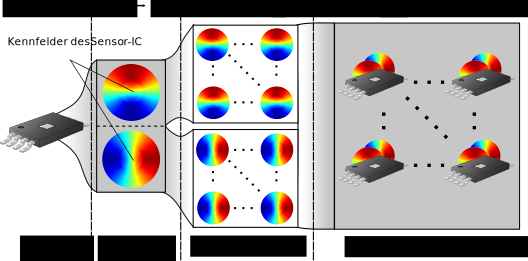
\includegraphics[width=\linewidth]{chapters/images/1-Motivation/Ansatz_Simulationsmodell}
	\caption[Ansatzdarstellung zur Generierung eines Simulationsmodell des magnetischen Sensor-Arrays]{Ansatzdarstellung zur Generierung eines Simulationsmodell des magnetischen Sensor-Arrays. Sensor spezifische Charakteristiken (Kennfelder) werden in einem Charakterisierungsdatensatz gespeichert und im Anschluss das Verhalten des Einzelexemplars zu einem Sensor-Array interpoliert. Die Simulation des interpolierten Sensor-Arrays erzeugt eine höhere Abstraktionsebene, deren Ergebnisse wiederum in Simulationsdatensätze gespeichert sind und zur weiteren Analyse und Evaluierung genutzt werden können. Die Abstraktion der Kennfelder soll hier das Prinzip des Simulationsansatzes veranschaulichen. Im Simulationsmodell werden keine Arrays von Kennfeldern aufgebaut, sondern Charakteristiken des einzelnen Kennfeldes entnommen und interpoliert. Die grau unterlegten Abschnitte kennzeichnen Verfahrensschritte, in denen Datensätze zur Verfügung stehen oder erzeugt werden.}
	\label{fig:ansatz-simulationsmodell}
\end{figure}


\clearpage


Das Sensor-Array-Modell, ob als Platinen-Modell oder Simulationsmodell, repräsentiert im Kontext nur die erste Hälfte 
eines modernen, vollwertigen Sensor-ICs. Seine Aufgabe besteht darin eine physikalische Anregung (Magnetfeld) in 
elektrische, analoge Signale umzuwandeln. Dieser Teil eines Sensor-ICs wird zumeist als \gls{gl:sensorkopf} bezeichnet, 
da eine sinnbildliche darunter liegende Einheit die weitere Signalverarbeitung und -Auswertung übernimmt. Es handelt 
sich dabei um eine anwendungsspezifische integrierte Schaltung, engl. \gls{ac:asic}. Beide Teile zusammen, der 
Sensorkopf und das Signalverarbeitungs-ASIC, bilden ein vollständiges Sensor-IC mit der Fähigkeit zur modernen 
Signalverarbeitung.
Unterstützend zeigt \autoref{fig:veranschaulichung-sensor-ic} die allgemeine Aufbaubeschreibung eines Sensor-IC und Unterteilung in Sensorkopf und ASIC, respektive Signalerzeugung und Signalverarbeitung.


\vspace{5mm}
\begin{figure}[tbph]
	\centering
	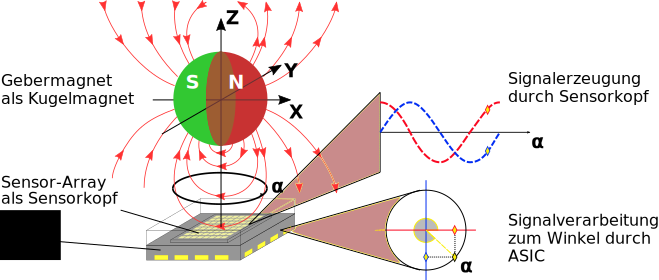
\includegraphics[width=\linewidth]{chapters/images/1-Motivation/Veranschaulichung_Sensor-IC}
	\caption[Veranschaulichung eines vollständigen Sensor-ICs für die Drehwinkelerfassung]{Veranschaulichung eines 
	vollständigen Sensor-ICs für die Drehwinkelerfassung. Stark vereinfachte Darstellung eines Sensor-IC bestehend aus 
	einem Sensorkopf und ASIC. Zu sehen sind die übergeordneten Aufgaben von Sensorkopf und ASIC. Der Sensorkopf 
	erfasst die physikalische Stimulanz (hier Kugelmagnetfeld) und setzt diese in analoge Signale um. Eine 
	anschließende Signalverarbeitung findet im ASIC statt, der die elektrischen Signal zur entsprechender Winkelausgabe 
	abstrahiert. Dargestellt ist die Signalerzeugung eines einzelnen Punktes auf dem magnetischen Sensor-Arrays. Grafik 
	entnommen und bearbeitet aus \cite{Schuethe2020}.}
	\label{fig:veranschaulichung-sensor-ic}
\end{figure}


\clearpage


\paragraph{ASIC - Konzeptionierung der Kernfunktionalität}\label{par:asic-konzeptionierung-der-kernfuntionalitaet}$~$\\


Derzeitig befinden sich die Forschungsprojektarbeiten für einen tauglichen ASIC in der Konzeptionsphase. Die Kernfunktionalität eines ASIC-Designs wird durch ein mathematisches Modell oder Verfahren abgebildet, dass in der Lage ist vom Sensorkopf erzeugte Messwerte adäquat und ausreichend schnell zu verarbeiten. Dabei muss ein solches Modell oder Verfahren grundlegende Eigenschaften des physikalischen Gesamtsystems in sich vereinigen und diese repräsentativ in den Gesamtkontext der Applikation setzen können. Im Kontext dieser Arbeit ist die Sensorapplikation, durch die Drehwinkelerfassung einer kreisförmigen Sensoranregung dargestellt, wie es in \autoref{fig:veranschaulichung-sensor-ic} angedeutet ist.

Erfolgte Vorarbeiten der \gls{gl:ags} für ein ASIC-Design, umfassen die Entwicklung eines mathematischen Modells und 
erste theoretische Simulationen \cite{Schuethe2019}\cite{Schuethe2020b}\cite{Schuethe2020}. Die Simulation bindet dabei Datensätze ein, die durch das Sensor-Array-Simulationsmodell erzeugt werden. Das mathematische Modell der ASIC-Kernfunktionalität ist auf Grundlage von Gauß-Prozessen für Regressionsverfahren entwickelt \cite{Rasmussen2006} worden. Die bisherigen Simulationsarbeiten beschränken sich auf mathematische Simulationen, die auf eine Gültigkeitsprüfung des mathematischen ASIC-Modells abzielen und Ansätze zur Modellqualifizierung und Qualitätskriterien für die Signalverarbeitung mit beinhalten.


\clearpage

